\chapter{Generalization of Dispersive Model for Multi Level Qubit}\label{appendix:multiqubit}
In section \ref{sec:dispersive_regime} the dispersive model was derived for 2-level-qubit. In this appendix, we will expand this to general form where we consider an m-level instead of the qubit. This derivation is based on the exercise from a ph.d. course in superconducting Qubits at the Niels Bohr Institute developed by Svend Krøjer \cite{kroejer_week_2023}. As earlier, we have energy for the resonator given by: $H_{res} = \omega_r a^\dagger a$ while the energy for an M-level qubit can be written generally as:
\begin{equation}
    H_{q} = \sum_{k = 0}^{M-1} \omega_k \ket{k}\bra{k}
\end{equation}
Where $\ket{k}$ is the k'th energy eigenstate of the qubit with corresponding energy of $\omega_k$. Allowing the M-level qubit to interact with the resonator by the Generalized Jaynes-Cumming model:
\begin{equation}
    H_1 =  \sum_{i,j} g_{ij} \ket{i}\bra{j} (a + a^\dagger ) 
\end{equation}
Where the jump strength $g_{ij}$ is related to the overlap of the eigenstates with the charge operator and the coupling energy: $g_{ij} = g \matrixel{i}{\hat{n}}{j}$. This gives the full Hamiltonian: 
% \begin{align}
%     H &= H_0 + H_1  \nonumber \\&= \omega_r a^\dagger a +  \sum_{k = 0}^{M-1} \omega_k \ket{k}\bra{k} + \sum_{i,j} g_{ij} \ket{i}\bra{j} (a + a^\dagger ) 
% \end{align}
\begin{fullwidth}
    \begin{equation}
        H = H_0 + H_1  = \omega_r a^\dagger a +  \sum_{k = 0}^{M-1} \omega_k \ket{k}\bra{k} + \sum_{i,j} g_{ij} \ket{i}\bra{j} (a + a^\dagger ) 
    \end{equation}
\end{fullwidth}
As in the two-level-system, we can make  use of the Schrieffer-Wolff transformation to diagonalize the Hamiltonian to second order in the perturbation variable. We want to apply the transfomration:
\begin{align}
    H' &= e^{S} H e^{-S} = H + \comm{S}{H} + \frac{1}{2}\comm{S}{\comm{S}{H}} + \dots \nonumber\\
                        &= H_0 + H_1 + \comm{S}{H_0 + H_1} + \frac{1}{2} \comm{S}{\comm{S}{H_0 + H_1}} + \dots
\end{align}
Where $S$ has to be an anti-hermitian operator to make this a unitary transformation. The goal is now to choose $S$ such that the linear terms in our perturbation disappear. This gives the condition $\comm{S}{H_0} = - H_1$. If we were to choose:
\begin{equation}
    S = \sum_{ij}g_{ij}\ket{i}\bra{j}\left(\frac{1}{\omega_{ij} - \omega_r}a + \frac{1}{\omega_{ij} + \omega_r} a^\dagger \right)
\end{equation}
with $\omega_{ij} = \omega_i - \omega_j$. The commutator gives:
\begin{fullwidth}
\begin{align*}
    \comm{S}{H_0} &= \sum_{ijk}g_{ij}\comm{\ket{i}\bra{j}\left(\frac{1}{\omega_{ij} - \omega_r}a + \frac{1}{\omega_{ij} + \omega_r} a^\dagger \right)}{\omega_r a^\dagger a + \omega_k \ket{k}\bra{k}} \\
    &= \sum_{ij} g_{ij}\ket{i}\bra{j} (\omega_j - \omega_i) \left(\frac{1}{\omega_{ij} - \omega_r}a + \frac{1}{\omega_{ij} + \omega_r} a^\dagger\right) \\
    &+ \sum_{ij} g_{ij} \ket{i}\bra{j} \omega_r \left(\frac{1}{\omega_{ij} - \omega_r} \comm{a}{a^\dagger a}  + \frac{1}{\omega_{ij} + \omega_r} \comm{a^\dagger}{a^\dagger a} \right) 
\end{align*}
\end{fullwidth}
And with $\comm{a^\dagger}{a^\dagger a} = - a^\dagger$ and $\comm{a^\dagger}{a a} = + a$. We obtain:
\begin{align*}
    &= \sum_{ij}g_{ij}\ket{i}\bra{j}\left(\frac{\omega_j - \omega_i - \omega_r}{\omega_{ij} + \omega_r} a + \frac{\omega_j - \omega_i - \omega_r}{\omega_{ij} + \omega_r} a^\dagger  \right) \\
    &= -\sum_{ij}g_{ij}\ket{i}\bra{j}(a + a^\dagger) = - H_1
\end{align*}
With this result, our transformed Hamiltonian now becomes:
\begin{align}
    H' &= H_0 + \comm{S}{H_1} + \frac12\comm{S}{\comm{S}{H_0 + H_1}} \dots \nonumber \\
       &= H_0 + \comm{S}{H_1} + \frac12\left( - \comm{S}{H_1} + \comm{S}{\comm{S}{H_1}}\right) \dots \\
       &= H_0 + \frac12\comm{S}{H_1} + \dots
\end{align}
In the dispersive limit, the coupling strength is much weaker than the detuning: $g_{ij} \ll w_{ij}$. Since S contains $g_{ij} / w_{ij}$ terms, we only go to the linear term in the dispersive approximation, and drop everything with higher orders of S. 

In this transformed basis, we find the "pertubation" entirely from: $H_{shift} = \frac12 \comm{S}{H_1}$ which can be calculated to:
\begin{fullwidth}
\begin{align*}
    2 H_{shift}&= \comm{\sum_{ij}g_{ij}\ket{i}\bra{j}\left(\frac{1}{\omega_{ij} - \omega_r}a + \frac{1}{\omega_{ij} + \omega_r} a^\dagger \right)}{\sum_{kl} g_{kl} \ket{k}\bra{l} (a + a^\dagger ) } \\
    &= \sum_{ijkl} g_{ij} g_{kl}\left[\ket{i}\delta_{jk}\bra{l}\left(\frac{1}{\omega_{ij} - \omega_r}a + \frac{1}{\omega_{ij} + \omega_r} a^\dagger \right)(a + a^\dagger)\right]\\
    &- \sum_{ijkl} g_{ij} g_{kl}\left[\ket{k} \delta_{li}\bra{j} (a + a^\dagger)\left(\frac{1}{\omega_{ij} - \omega_r}a + \frac{1}{\omega_{ij} + \omega_r} a^\dagger\right)\right]
\end{align*}
\end{fullwidth}
Going into the rotating frame terms proportional to $aa$ or $a^\dagger a^\dagger$ will be negligible since they are not energy conserving. Furthermore, the Scrieffer Wolf diagonalized to first order, so we will only keep diagonal elements proportional to $\ket{i}\bra{i}$. We find:
\begin{fullwidth}
\begin{align*}
    2 H_{shift} &= \sum_{ij} |g_{ij}|^2 \ket{i}\bra{i} \left[\frac{1}{\omega_{ij} - \omega_r}aa^\dagger - \frac{1}{\omega_{ji} + \omega_r} a^\dagger a + \frac{1}{\omega_{ij} - \omega_r}a^\dagger a - \frac{1}{\omega_{ji} + \omega_r}  a a^\dagger  \right]
\end{align*}
\end{fullwidth}

Using the commutation relation $\comm{a}{a^\dagger} = 1$, we can write it in the following form:
\begin{fullwidth}
\begin{equation}
    H_{shift} = \sum_{ij} \ket{i}\bra{i} |g_{ij}|^2 \left(\frac{1}{\omega_{ij} - \omega_r} + \left(\frac{1}{\omega_{ij} - \omega_r} + \frac{1}{\omega_{ij} + \omega_r} \right)a^\dagger a\right)
\end{equation}
\end{fullwidth}

And by defining the following quantities:
\begin{align}
    \chi_{ij} &= |g_{ij}|^2 \left(\frac{1}{\omega_{ij} - \omega_r} + \frac{1}{\omega_{ij} + \omega_r} \right) \\
    \delta_{ij} &= \frac{|g_{ij}|^2 }{\omega_{ij} - \omega_r} \\
    \chi_{i} &= \sum_j \chi_{ij} \\
    \delta_{i} &= \sum_j \delta_{ij} 
\end{align}
The dispersive m-level qubit and resonator system can be written as:
\begin{equation}
    H' = \omega_r a^\dagger a + \sum_k \omega_k \ket{k}\bra{k} + \sum_{kl}\ket{k}\bra{k}(\delta_{kl} + \chi_{kl} a^\dagger a )
\end{equation}
Or in a more interpretable manner:
\begin{equation} \label{eq:multi_qubit_dispersive_hamiltonian}
    H' = \left(\omega_r + \sum_k \chi_k \ket{k}\bra{k} \right) a^\dagger a + \sum_k (\omega_k + \delta_k)\ket{k}\bra{k}
\end{equation}
This equation allows us to investigate the effect of the coupling between resonator and qubit. When coupled the qubit state shift the resonator frequency with $\chi_k$. While every qubit frequency is shifted slightly y $\delta_k$.

% \begin{marginfigure}
%     \centering
%     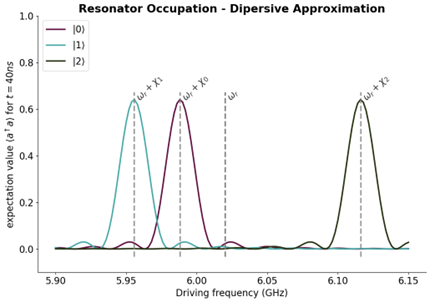
\includegraphics{Figs/Sections/computations_and_readout/three_qubit_states_dispersive.png}
%     \caption{Driving the resonator will show resonance around a frequency determined by the qubit state. For a three state qubit the above is found:}
%     \label{fig:three_state_dispersive}
% \end{marginfigure}

Or by considering reducing the multi-level system to only the two lowest, we can write the equation in the simple form:
\begin{equation}\label{eq:two_level_qubit_dispersive}
    H = (\Tilde{\omega}_r + \chi \sigma_z) a^\dagger a + \frac12 \Tilde{\omega}_{01} \sigma_z
\end{equation}
where the shifts from the higher order terms have been absorbed into the new redefined frequencies.
% Altering the dispersive shift to the type\cite{krantz_quantum_2019}: 
% \begin{equation}
%     \chi = \chi_{01} + \chi_{12}/2 = - g_{01}^2/\Delta \left(\frac{1}{1 + \Delta / \alpha}\right)
% \end{equation}

% Maybe comment on resonator critical photon count here. \todo{Would be nice... }
